\documentclass{beamer}

\usepackage{beamerthemeCopenhagen}
%\usepackage{beamerthemeBerkeley}
%\usepackage{beamercolorthemeseahorse}
%\usepackage{color}
\usepackage{hyperref}
\usepackage{graphicx}
\usepackage[brazil]{babel}
\usepackage[latin1]{inputenc}
\usepackage{listings,color,textcomp}
%\definecolor{listinggray}{gray}{0.3}
\definecolor{lbcolor}{rgb}{0.9,0.9,0.9}
\lstset{
	backgroundcolor=\color{white},
	tabsize=4,
	rulecolor=,
	language=Perl,
    basicstyle=\scriptsize,
    upquote=true,
    aboveskip={1.5\baselineskip},
    columns=fixed,
    showstringspaces=false,
    extendedchars=true,
    breaklines=true,
    prebreak = \raisebox{0ex}[0ex][0ex]{\ensuremath{\hookleftarrow}},
    frame=shadowbox,
    showtabs=false,
    showspaces=false,
    numbers=left,
    showstringspaces=false,
    identifierstyle=\ttfamily,
    keywordstyle=\color[rgb]{0,0,1},
    commentstyle=\color[rgb]{0.133,0.545,0.133},
    stringstyle=\color[rgb]{0.627,0.126,0.941},
}
\logo{
\includegraphics[scale=0.3]{yapc.png}}
%\logo{YAPC::Brasil::2009}

\title{Perl para \textit{Sysadmins} e \textit{DBA's}}
\author{Lindolfo ''Lorn'' Rodrigues}
\date{}

\begin{document}

\beamertemplatetransparentcoveredmedium

\frame{\titlepage}

%\begin{frame}[shrink]
%\tableofcontents
%\end{frame}

\section{Introdu��o}

\frame 
{
  \frametitle{\$ whoami}
  %\lstinputlisting{foo.pl}
  \$ id 

  \$ uid=1000(lorn) gid=100(users)

  grupos=11(\#sao-paulo.pm), 17(\#slackware-br), 18(\#catalyst), 19(\#moose),83(\#perl6)

}


\frame 
{
  \frametitle{Agenda}

  \begin{itemize}[<+->]
  \item \textit{Sysadmin}  
  \begin{itemize}[<+->]
    \item One-liners
    \item Parsers de log
    \item Automatiza��es
  \end{itemize}
  \end{itemize}
  \begin{itemize}[<+->]
  \item \textit{DBA}
  \begin{itemize}[<+->]
    \item ETL
    \item Data Cleaning
  \end{itemize}
  \end{itemize}

}


\section{Sysadmin}


\frame
{
  \frametitle{One-liners}
  \begin{itemize}[<+->]
    \item Perl na linha de comando
    \item Lembra muito sed/awk, com todo o poder da PCRE
  	\begin{itemize}[<+->]
   	 \item sed: sed -i.bck -e 's/foo/bar/g' arquivo.txt
   	 \item perl: perl -i.bck -npe 's/foo/bar/g' arquivo.txt
  	\end{itemize}
  	\begin{itemize}[<+->]
   	 \item awk: awk '\{print \$1;\}' arquivo.txt
   	 \item perl: perl -npe 'print \$F[0]' arquivo.txt
  	\end{itemize}
	\item Perl = Shell Script + awk + sed + ... + CPAN! \\o/
  \end{itemize}
}


\frame
{
  \frametitle{One-liners}

  \begin{itemize}[<+->]
    \item find /var/www -iname "*.html" -exec perl -i.bck -npe 's/foo/bar/g' '{}' \;
	\item perl -MDBD::mysql -e 'DBD::mysql->connect('dbname=yapc;Host=192.168.1.2', 'root', 'yapc2009')
  \end{itemize}
}

\frame
{
  \frametitle{One-liners}
  \begin{itemize}[<+->]
    \item dicas.txt ( canivete sui�o one-liners )
	\item App::Rad!
  \end{itemize}
}


\frame
{
  \frametitle{One-liners}
  \lstinputlisting{rad.pl}
}


\frame
{
  \frametitle{One-liners}
  \begin{itemize}[<+->]
  	\item \$ perl dicas.pl include 'arruma\_string' -i.bck -npe 's/foo/bar/g' arquivo.txt
  	\item \$ perl dicas.pl 
	\lstinputlisting{rad.txt}
	\item \$ perl dicas.pl arruma\_string outro\_arquivo.txt
  \end{itemize}
}


\frame
{
  \frametitle{One-liners}
  \begin{figure}[h]
    \centering
    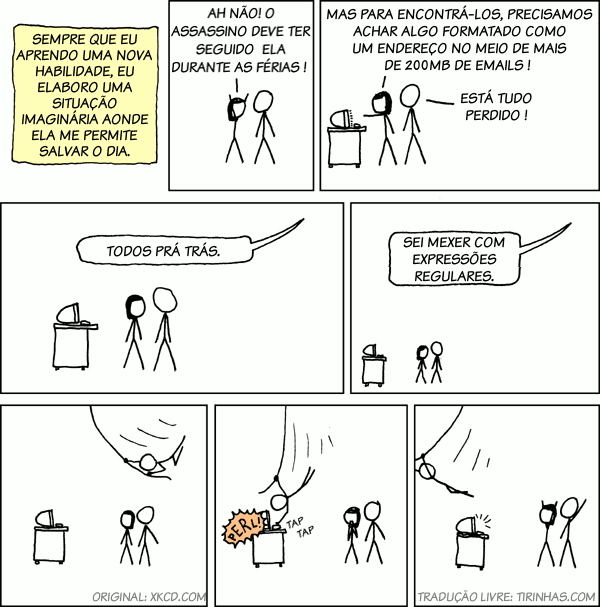
\includegraphics [scale=0.28]{perl_xkcd.png}
  \end{figure}
}


\frame
{
  \frametitle{Parsers}
  \begin{itemize}[<+->]
  \item Como mandar o log do Apache para o Syslog ( tutorial no ultimo slide ) 
  \item PABX
  \begin{itemize}[<+->]
  	\item Usar Spreadsheet::Write
	\item Customizar com cores, gerentes/chefes adoram cores
  \end{itemize}
  \item maillog
  \end{itemize}
}

\frame 
{
  \frametitle{Pr�-requisitos}
  Hash tables, o que s�o e como pode ser usada?
  \frametitle{Pr�-requisitos}
  \lstinputlisting{hash.pl}

}

\frame 
{
  \frametitle{Pr�-requisitos}
  Estrutura de um hash:
  \lstinputlisting{dump.txt}
}


\frame
{
  \frametitle{Pega ''spider''}
  Pegando o ''invasor'' do seu site
  \lstinputlisting{conta_acessos.pl}
}

\frame
{
  \frametitle{Pega ''spider''}
  \lstinputlisting{acessos.txt}
}

\frame
{
  \frametitle{Achando arquivo duplicados}
  \lstinputlisting{duplicados.pl}
}

\frame
{
  \frametitle{Achando arquivo duplicados}
  \lstinputlisting{duplicados2.pl}
}


\frame
{
  \frametitle{Achando arquivo duplicados}
  \lstinputlisting{md5.txt}
}

\frame
{
  \frametitle{Automatizando tarefas}
  \begin{itemize}[<+->]
  \item Qualquer programa com opcao de include, pode ser automatizado 
  \item Apache, Samba, Bind
  \end{itemize}
}

\section{DBA}

\frame
{
  \frametitle{Extract, transform, loading}
  \begin{itemize}[<+->]
  \item Nenhuma linguagem carrega dados no banco, mais rapido que o proprio banco
  \item pg\_copy ( PostgreSQL ) , impdmp ( Oracle ) 
  \item ..mas voc� pode modificar o que ser� carregado antes de usar o proprio banco
  \item Limpeza de caracteres '?' 
  \item dupla dinamic ord - chr
  \begin{itemize}[<+->]
 	\item ord: descobre o ''id'' do caracter estranho
	\item chr: recebe o ''id'' do caracter e retorna o mesmo
	\item my \$id\_estranho = ord(371); 
	\item my \$char\_estranho = chr(\$id\_estranho);
	\item my \$texto\_sujo =~ s/\$char\_estranho//g;
  \end{itemize}
  \item Validar os dados de entrada ( CNPJ, CPF, etc )
  \item Business::BR::CNPJ Business::BR::CPF 
  \end{itemize}
}


\frame
{
  \frametitle{Extract, transform, loading}
  \begin{itemize}[<+->]
  \item Spreadsheet::Write tamb�m funciona bem com SELECT
  \item ... ou seja, n�o precisa gerar um .csv e carregar no seu ''Excel''
  %\item SELECT to XLS, ou como deixar seus chefes mais felizes :)
  \item ..mas voc� pode modificar o que ser� carregado antes de usar o proprio banco
  \end{itemize}
}

\frame
{
  \frametitle{Extract, transform, loading}
  \begin{itemize}[<+->]
  \item Pequel ETL 
  \end{itemize}
}

\frame
{
  \frametitle{PL/Perl - PL/PerlU}
  \begin{itemize}[<+->]
  \item Palesta do David Fetter ( http://fetter.org ) 
  \end{itemize}
}

\frame
{
  \frametitle{Data Cleaning}
  \begin{itemize}[<+->]
  \item Text::Levenshtein ( Edit Distance ou Levenshtein Distance )
  \begin{itemize}[<+->]
  	\item rato - ralo
	\item rodar - rodo
  \end{itemize}
  \item Algorithm::LCS
  \item Algoritmo usado no diff de codigos
  \end{itemize}
}

\section{Considera��es finais}

\frame
{
	\frametitle{Bibliografia e coisas interessantes}
    \href{http://www.ibm.com/developerworks/linux/library/l-punix.html}{Cultured
    Perl: Automating UNIX system administration with Perl}

    \href{http://www.ibm.com/developerworks/linux/library/l-p101/}{Cultured
    Perl: One-liners 101}

    \href{http://www.oreillynet.com/pub/a/sysadmin/2006/10/12/httpd-syslog.html}{Sending
    Apache httpd Logs to Syslog}

    \href{http://www.lornlab.org/palestra\_yapc2009}{http://www.lornlab.org/
    palestra\_yapc2009/}
}


\frame
{
  \frametitle{Obrigado}
  \begin{itemize}[<+->]
  \item Duvidas?
  \item lorn@lornlab.org
  \end{itemize}
}




\end{document}
